%%%%%%%%%%%%%%%%%%%%%%%%%%%%%%%%%% Chapter 6 %%%%%%%%%%%%%%%%%%%%%%%%%%%%%%%%%%
\chapter{Implementation \label{chapter:6}}
    This chapter will explain the code used in the thesis in detail. The code
    itself i given in >> REF GITHUB REPO <<. General information of the usage
    of packages are given in appendix >> REF APPENDIX << while the structure
    and workflow of the code is given here. Theory backing the implementation
    is given in >> REF THEORY CHAPTER <<

\section{Cartesian Basis}
    In \Arf{chapter:4} we mentioned the use of basis functions the different
    Many-Body methods. These can be pre-built using nifty intuition. One such
    observation is in the way harmonic oscillator functions station themselves
    on energy-levels(in the full-shell case). The following image\footnote{As
    the old idiom goes; "A picture is worth a thousand words"} describes this
    for the first few levels
        \begin{figure}[H]
            \centering
            \begin{subfigure}[b!]{0.49\textwidth}
                \centering
                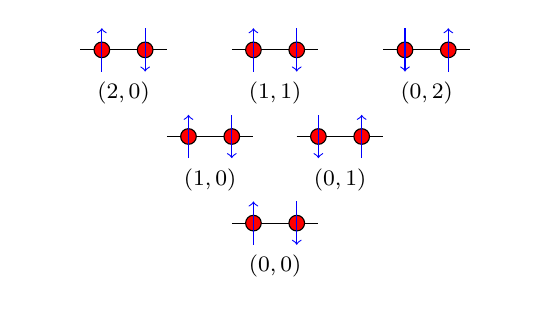
\begin{tikzpicture}[scale=0.55]
                    \draw (-1,0) -- (1,0);
                    \node at (-0.5,0) [draw,circle,fill=red,scale=0.6] {};
                    \node at (0.5,0) [draw,circle,fill=red,scale=0.6] {};
                    \draw[blue, ->] (-0.5,-0.5) -- (-0.5,0.5);
                    \draw[blue, <-] (0.5,-0.5) -- (0.5,0.5);
                    \node[text width=2.2cm, align=center] at (0,-1) {\footnotesize{$(0,0)$}};
                    \draw (-2.5,2) -- (-0.5,2);
                    \node at (-2.0,2) [draw,circle,fill=red,scale=0.6] {};
                    \node at (-1.0,2) [draw,circle,fill=red,scale=0.6] {};
                    \draw[blue, ->] (-2.0,1.5) -- (-2.0,2.5);
                    \draw[blue, <-] (-1.0,1.5) -- (-1.0,2.5);
                    \node[text width=2.2cm, align=center] at (-1.5,1) {\footnotesize{$(1,0)$}};
                    \draw (0.5,2) -- (2.5,2);
                    \node at (1.0,2) [draw,circle,fill=red,scale=0.6] {};
                    \node at (2.0,2) [draw,circle,fill=red,scale=0.6] {};
                    \draw[blue, <-] (1.0,1.5) -- (1.0,2.5);
                    \draw[blue, ->] (2.0,1.5) -- (2.0,2.5);
                    \node[text width=2.2cm, align=center] at (1.5,1) {\footnotesize{$(0,1)$}};
                    \draw (-4.5,4) -- (-2.5,4);
                    \node at (-4.0,4) [draw,circle,fill=red,scale=0.6] {};
                    \node at (-3.0,4) [draw,circle,fill=red,scale=0.6] {};
                    \draw[blue, ->] (-4.0,3.5) -- (-4.0,4.5);
                    \draw[blue, <-] (-3.0,3.5) -- (-3.0,4.5);
                    \node[text width=2.2cm, align=center] at (-3.5,3) {\footnotesize{$(2,0)$}};
                    \draw (-1,4) -- (1,4);
                    \node at (-0.5,4) [draw,circle,fill=red,scale=0.6] {};
                    \node at (0.5,4) [draw,circle,fill=red,scale=0.6] {};
                    \draw[blue, ->] (-0.5,3.5) -- (-0.5,4.5);
                    \draw[blue, <-] (0.5,3.5) -- (0.5,4.5);
                    \node[text width=2.2cm, align=center] at (0,3) {\footnotesize{$(1,1)$}};
                    \draw (4.5,4) -- (2.5,4);
                    \node at (4.0,4) [draw,circle,fill=red,scale=0.6] {};
                    \node at (3.0,4) [draw,circle,fill=red,scale=0.6] {};
                    \draw[blue, ->] (4.0,3.5) -- (4.0,4.5);
                    \draw[blue, <-] (3.0,3.5) -- (3.0,4.5);
                    \node[text width=2.2cm, align=center] at (3.5,3) {\footnotesize{$(0,2)$}};
                \end{tikzpicture}
                \caption{Two-dimensional case with $(n_x,n_y)$ notation.}
                \label{subfig:2Dspin}
            \end{subfigure}
            \begin{subfigure}[b!]{0.49\textwidth}
                \centering
                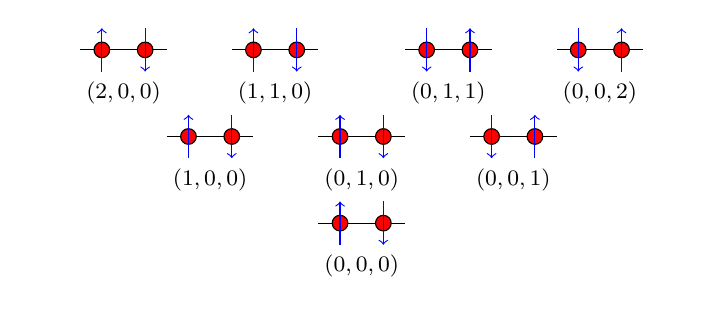
\begin{tikzpicture}[scale=0.55]
                    \draw (-1,0) -- (1,0);
                    \node at (-0.5,0) [draw,circle,fill=red,scale=0.6] {};
                    \node at (0.5,0) [draw,circle,fill=red,scale=0.6] {};
                    \draw[blue, ->] (-0.5,-0.5) -- (-0.5,0.5);
                    \draw[blue, <-] (0.5,-0.5) -- (0.5,0.5);
                    \node[text width=3.5cm, align=center] at (0,-1) {\footnotesize{$(0,0,0)$}};
                    \draw (-4.5,2) -- (-2.5,2);
                    \node at (-4.0,2) [draw,circle,fill=red,scale=0.6] {};
                    \node at (-3.0,2) [draw,circle,fill=red,scale=0.6] {};
                    \draw[blue, ->] (-4.0,1.5) -- (-4.0,2.5);
                    \draw[blue, <-] (-3.0,1.5) -- (-3.0,2.5);
                    \node[text width=2.2cm, align=center] at (-3.5,1) {\footnotesize{$(1,0,0)$}};
                    \draw (-1,2) -- (1,2);
                    \node at (-0.5,2) [draw,circle,fill=red,scale=0.6] {};
                    \node at (0.5,2) [draw,circle,fill=red,scale=0.6] {};
                    \draw[blue, ->] (-0.5,1.5) -- (-0.5,2.5);
                    \draw[blue, <-] (0.5,1.5) -- (0.5,2.5);
                    \node[text width=2.2cm, align=center] at (0,1) {\footnotesize{$(0,1,0)$}};
                    \draw (2.5,2) -- (4.5,2);
                    \node at (3.0,2) [draw,circle,fill=red,scale=0.6] {};
                    \node at (4.0,2) [draw,circle,fill=red,scale=0.6] {};
                    \draw[blue, <-] (3.0,1.5) -- (3.0,2.5);
                    \draw[blue, ->] (4.0,1.5) -- (4.0,2.5);
                    \node[text width=2.2cm, align=center] at (3.5,1) {\footnotesize{$(0,0,1)$}};
                    \draw (-6.5,4) -- (-4.5,4);
                    \node at (-6.0,4) [draw,circle,fill=red,scale=0.6] {};
                    \node at (-5.0,4) [draw,circle,fill=red,scale=0.6] {};
                    \draw[blue, ->] (-6.0,3.5) -- (-6.0,4.5);
                    \draw[blue, <-] (-5.0,3.5) -- (-5.0,4.5);
                    \node[text width=2.2cm, align=center] at (-5.5,3) {\footnotesize{$(2,0,0)$}};
                    \draw (-3.0,4) -- (-1.0,4);
                    \node at (-2.5,4) [draw,circle,fill=red,scale=0.6] {};
                    \node at (-1.5,4) [draw,circle,fill=red,scale=0.6] {};
                    \draw[blue, ->] (-2.5,3.5) -- (-2.5,4.5);
                    \draw[blue, <-] (-1.5,3.5) -- (-1.5,4.5);
                    \node[text width=2.2cm, align=center] at (-2.0,3) {\footnotesize{$(1,1,0)$}};
                    \draw (3.0,4) -- (1.0,4);
                    \node at (2.5,4) [draw,circle,fill=red,scale=0.6] {};
                    \node at (1.5,4) [draw,circle,fill=red,scale=0.6] {};
                    \draw[blue, ->] (2.5,3.5) -- (2.5,4.5);
                    \draw[blue, <-] (1.5,3.5) -- (1.5,4.5);
                    \node[text width=2.2cm, align=center] at (2.0,3) {\footnotesize{$(0,1,1)$}};
                    \draw (6.5,4) -- (4.5,4);
                    \node at (6.0,4) [draw,circle,fill=red,scale=0.6] {};
                    \node at (5.0,4) [draw,circle,fill=red,scale=0.6] {};
                    \draw[blue, ->] (6.0,3.5) -- (6.0,4.5);
                    \draw[blue, <-] (5.0,3.5) -- (5.0,4.5);
                    \node[text width=2.2cm, align=center] at (5.5,3) {\footnotesize{$(0,0,2)$}};
                \end{tikzpicture}
                \caption{Three-dimensional case with $(n_x,n_y,n_z)$ notation.}
                \label{subfig:3Dspin}
            \end{subfigure}
            \caption{Harmonic Oscillator Levels}
            \justify
        \end{figure}
    This specific arrangement of basis-functions is implemented in class
    \hltexttt{Cartesian} and is used in both the Hartree-Fock and VMC
    implementations. It essentially builds a matrix of states with the rows
    being the specific state and the columns containing the quantum numbers(in
    cartesian), the spin-value(as an integer), magic number and energy(in
    natural units proportional to the oscillator frequency). The essential form
    is
        \begin{equation}
            \begin{aligned}
                \begin{pmatrix}
                    n_x & n_y & s & m_s & E & M
                \end{pmatrix}
                \indent
                \begin{pmatrix}
                    n_x & n_y & n_z & s & m_s & E & M
                \end{pmatrix}
            \end{aligned}
        \end{equation}
    with the $n$'s being the principal numbers, $s$ the spin value $m_s$ the
    spin projection(up or down in our case), $E$ the energy and $M$ the magic
    number. The \hltexttt{Cartesian} class builds the states with alternating
    spin (the spacial parts are doubled with spin), but also has a function for
    restructuring by setting the states with spin down in acending order first
    and the same states with spin up after.

\section{Hartree-Fock}
    The Hartree-Fock method described in \Arf{sec:HFtheory} is implemented in
    >> REF GITHUB <<. Only the restricted case is implemented and is present as
    the class \hltexttt{HartreeFockSolver}. The matrix-elements(integrals) are
    implemented in \hltexttt{HermiteIntegrals} class. This class also uses an
    auto-generated header for the Hermite-coefficients, see
    \Arf{sec:auto_generation} below. The \hltexttt{HartreeFockSolver} is
    implemented in a general way such that an abstract class for the integral
    elements is all that is needed. The \hltexttt{HartreeFockSolver} can then
    be inherited and used.  An example of how to create a solver object with
    the Double-Well system called HFS with number of dimensions $D$, number of
    basis functions $L$ and number of particles $N$.
        \begin{lstlisting}[language=C++, style=ccstyle]
            DoubleWell* HFS = new DoubleWell(D, L, N);
            string message = HFS->initializeParameters(...);
        \end{lstlisting}
    With the $\dots$ meaning one initializes it with in however manner the
    function was made. The initialization function must also return a message
    determined by the success of the initialization. If it succeeds it return
    an empty message while if not it returns a pre-defined message. \\ 
    Here is a simple example code-snippet which initializes and runs the
    Hartree-Fock algorithm
        \begin{lstlisting}[language=C++, style=ccstyle]
            DoubleWell* HFS = new DoubleWell(D, L, N);

            string message = HFS->initializeParameters(...);
            if (message.compare("")) {
                if (myRank == 0) {
                    std::cout << message << std::endl;
                } // end if
                delete HFS;
                finalize();
            } // end if

            double E = HFS->iterate(M, 1e-8, true);
        \end{lstlisting}
    The \hltexttt{iterate} function takes in $M$ as the maximum number of
    iterations, the convergence tolerance (when to break the iteration) and a
    boolean for showing progress or not. It calculates the integral-elements
    and runs the Hartree-Fock algorithm and returns the estimation of the
    ground-state energy.

\subsection{Parallelization of Two-Body Matrix}
    The most time-consuming part of the Hartree-Fock procedure is the
    calculation of the two-body matrix-elements giving the interaction terms.
    This is parallelized in the \hltexttt{assemble} function in
    \hltexttt{HartreeFockSolver}. The basic premise is to represent the $N^4$
    elements $\Braket{pq|r^{-1}|rs}$ as a one-dimensional array with the mapping
        \begin{equation}
            (p,q,r,s) \rarr p + N(q + N(r + Ns))
        \end{equation}
    that is the element $(p,q,r,s)$ is stored in position $(p + N(q + N(r +
    Ns))$ in the one-dimensional array. The symmetry $(p,q,r,s)=(q,p,r,s)$
    reduces the number of elements down to $N(N+1)/2$. A $N(N+1)/2\times 4$
    matrix of indices is then created with
        \begin{algorithm}[H]
            \caption{Parallelization Index Mapping}\label{alg:paraindiexmap}
            \begin{algorithmic}[H]
                \State Initialize matrix pqMap with $\frac{N}{2}(N+1)$ rows and
                $4$ columns.
                \State j = 0
                \For{p=0 : N-1}
                    \For{q=p : N-1}
                        \For{r=0 : N-1}
                            \For{s=r : N-1}
                                \State pqMap[j,0] = p
                                \State pqMap[j,1] = q
                                \State pqMap[j,2] = r
                                \State pqMap[j,3] = s
                                \State j = j + 1
                            \EndFor
                        \EndFor
                    \EndFor
                \EndFor
            \end{algorithmic}
        \end{algorithm}
    The rows are then distributed evenly among $P$ processes according to
        \begin{equation}
            \text{rows} = \left\{\begin{aligned}
                \left\lceil\frac{\frac{N^2}{4}(N+1)^2}{P}\right\rceil &\indent&
                &\text{rank} < \left(\frac{N^2}{4}(N+1)^2\mod P\right) \\
                \left\lfloor\frac{\frac{N^2}{4}(N+1)^2}{P}\right\rfloor
                &\indent& &\text{else}
                \end{aligned}\right.
        \end{equation}
    The problem now however is that processes of higher and higher ranks my end
    up with calculating more since larger indices involve computationally more
    heavy functions to be evaluated. We can account for this by weighting the
    number of rows each process gets by the sum of the indices. The algorithm
    is as follows
        \begin{algorithm}[H]
            \caption{Even Weighting}\label{alg:parasumweight}
            \begin{algorithmic}[H]
                \State Make array $S$ of size $P$ with each element being the
                sum of the $(p,q,r,s)$ elements for the specific process.
                \State Make an array sizes of size $P$ with the number of
                elements for each process.
                \State Make an array displ of size $P$ with the displacement
                (index).
                \State $O =$ Mean of $S$.
                \For{$i=0$ to $P-2$}
                    \For{$j=$displ$[i]$ to displ$[i]+$sizes$[i+1]$} 
                    \Comment{Iterate over elements in right adjacent process.}
                        \State $L = S[i] + $sum(pqMap.row($j$))
                        \If{$L < O$}
                            \State sizes$[i] =$ sizes$[i] + 1$
                            \State sizes[$i+1$] = sizes[$i+1$]$ - 1$;
                            \State displ[$i+1$] = displ[$i+1$]$ + 1$;
                        \ElsIf{$L$ equals $O-1$ or $L$ equals $O+1$ or $L>O$}
                            \State Break inner-most loop.
                        \EndIf
                    \EndFor
                    \State Set elements of $S$.
                \EndFor
            \end{algorithmic}
        \end{algorithm}
    Each process has access to the \hltexttt{pqMap} array such that the each
    process calculates its own chunk according to the size set and the
    \hltexttt{displ} tells the start-index. Each process then calculates the
    two-body elements according to
        \begin{algorithm}[H]
            \caption{Two-Body Calculation}\label{alg:paratwobody}
            \begin{algorithmic}[H]
                \State Initialize $A$ for containing $(p,q,r,s)$ elements.
                \State Initialize $B$ for containing $(p,q,s,r)$ elements.
                \State $i_{\text{start}} =$ displ[rank]
                \State $i_{\text{end}} =$ displ[rank] $+$ sizes[rank]
                \State $k=0$
                \For{$l=i_{\text{start}}$ to $i_{\text{end}}-1$}
                    \State $p=$pqMap$[l,0]$
                    \State $q=$pqMap$[l,1]$
                    \State $r=$pqMap$[l,2]$
                    \State $s=$pqMap$[l,3]$
                    \State $A[l]=\Braket{pq|\frac{1}{r_{12}}|rs}$
                    \State $B[l]=\Braket{pq|\frac{1}{r_{12}}|sr}$
                \EndFor
            \end{algorithmic}
        \end{algorithm}
    Each $A$ and $B$ is then sent to root process and concatenated to a large
    one-dimensional array and the actual two-body matrix of size $N^4$ is
    assembled and antisymmetrized. The Hartree-Fock algorithm is then run only
    on one process.
    
    >> make structure (image??) of HartreeFock::All structure)

\section{Variational Monte Carlo}
    The Variational Monte-Carlo implementation is mainly in three classes,
    namely \hltexttt{VMC}, \hltexttt{BruteForce} and
    \hltexttt{ImportanceSampling}. The structure is set such that both
    \hltexttt{BruteForce} and \hltexttt{ImportanceSampling} inherit
    \hltexttt{VMC}. This structure essentially gives room for splitting
    specific part of the Brute-Force algorithm from the Metropolis-Hastings
    algorithm, but still using the same code for minimization. We will explain
    the minimization parts in the next section. \\ The main input which
    \hltexttt{VMC} needs is a wavefunction. An abstract class-template is
    implemented and can be generated using a python script, also given in the
    same GitHub repository >>REF GITHUB <<. The template is built in such a way
    that one only needs to fill in specific analytic expressions for the
    gradient, Laplacian and gradient for the variational parameters. The latter
    part is optional. \\ The wavefunction itself is built using the
    \hltexttt{Slater} or \hltexttt{SlaterJastrow} class. However, in order to
    use the \hltexttt{SlaterJastrow} one has to specify which Jastrow function
    to use at compile time. A simple example illustrates this in detail >> MAKE THIS EXAMPLE <<

    >> explain Jastrow classes
    >> make structure (image??) of VMC structure)

\section{Minimization}
\subsection{More-Thuente Linesearch}
\subsection{Conjugate Gradient}
\subsection{BFGS}
\section{Auto-Generation\label{sec:auto_generation}}
    The analytic expressions involved in the quantum-dot systems are dependent
    on Hermite-Polynomials and their coefficients. These are calculated
    symbolically using the recurrence relation for Hermites with the SymPy
    package in python. These expressions are then written to \CC code and
    written to a \CC-header file. This file is then included in the integral
    class in \hltexttt{HartreeFockSolver} and in the wavefunction
    classes(namely \hltexttt{HartreeFock} and \hltexttt{HarmonicOscillator}) in
    \hltexttt{VMC}. >> REF GITHUB <<
\section{Verification\label{sec:verification}}

    >> tables
